\documentclass[12pt,a4paper]{article}
\usepackage[utf8]{inputenc}
\usepackage[finnish]{babel}
\usepackage{setspace}
%\usepackage{parskip}
%\usepackage{amssymb}
%\usepackage{amsmath}
\usepackage{graphicx}
\usepackage{subcaption}
\usepackage{fancyhdr}
\usepackage[top=1in, bottom=1in, left=1in, right=1in]{geometry}
\usepackage{float}
\usepackage[section]{placeins}
\usepackage[nottoc,notlot,notlof]{tocbibind}
%\usepackage{listings}

\usepackage{titlesec}
\titleclass{\section}{top}
\newcommand\sectionbreak{\clearpage}
\titleformat*{\section}{\Huge\bfseries}
\titleformat*{\subsection}{\Large\bfseries}
\titleformat*{\subsubsection}{\large\bfseries}

%\usepackage[numbered,autolinebreaks,useliterate]{mcode}

\usepackage{siunitx}\sisetup{per=frac} % SI-yksiköitä.
%\usepackage{supertabular} % jos tarttee isoja taulukoita

\usepackage{hyperref}
\hypersetup{pdfborder={0 0 0}}
\onehalfspacing
\cfoot{}
\setlength{\parindent}{0pt}
\newcommand{\yt}{\texttt{yt}}


\begin{document}

% Sisällysluettelo
\newpage
\thispagestyle{empty}
\tableofcontents
\newpage
\setcounter{page}{1}
\parskip=1em \advance\parskip by 0pt plus 2pt
\pagestyle{fancy}
\cfoot{\thepage}

%%%%%%%%%%%%%%% Oleellinen sisältö alkaa%%%%%%%%%%%%%%%
\section{Johdanto}
\cite{rj, yt, enzo} %TODO http://arxiv.org/pdf/astro-ph/0403044v1.pdf hyvä soossi

%Teoreettista teoriaa. Täällä tarvitaan myös yhtälöitä, yhtälö \ref{esimerkkiyhtalo} on yksi sellainen.
%
%\begin{equation}\label{esimerkkiyhtalo}
%	c=\sqrt{a^2+b^2}
%\end{equation}

%\begin{align} % &-merkki kertoo mitkä kohdat laitetaan päällekkäin
%s_{1} =& d \cos \alpha = d \cos (90 \,^{\circ} - \varphi) = d \sin \varphi \label{align1} \\
%s_{2} =& d \cos \beta = d \cos (90 \,^{\circ} - \theta) = d \sin \theta \label{align2},
%\end{align}
%\begin{align}
%\lambda&=\frac s n \nonumber \\
%&= \frac{s_1-s_2}{n} \nonumber \\
%&= \frac{d}{n} ( \sin \varphi - \sin \theta ) \label{sievennystulos}
%\end{align}

%\begin{equation*}
%	\sin{x} \approx x \text{ kun x on pieni}
%\end{equation*}


\section{Enzo}
Enzo on astrofysikaalisten fluidien simulointiin käytettävä ilmainen ja avoin simulaatiokoodi, joka on suunniteltu kosmologisten rakenteiden simulointiin. Se tukee muun muassa hydrodynamiikkaa, ideaalista ja epäideaalista magnetohydrodynamiikkaa, N kappaleen simulaatioita, kaasupilvien kemiaa, säteilynkuljetusta, tähtien syntyä sekä maailmankaikkeuden laajenemista. \cite{enzo} %TODO tukeminen tyhmästi sanottu

Enzo hyödyntää mukautuvaa hilantihennystä (\textit{Adaptive Mesh Refinement}, AMR), joka mahdollistaa aika- ja paikkaresoluution kasvattamisen simulaation kiinnostavilla alueilla. Tämä on tärkeää, sillä usein melko pienellä alueella tarvitaan suurta resoluutiota, mutta koko simulaation ajaminen näin suurella tarkkuudella veisi kohtuuttoman paljon aikaa. \cite{enzo}

\subsection{Hila}
Simuloitava alue katetaan kokonaan hilalla, jonka tiheys valitaan sellaiseksi, että saavutetaan pienin haluttava resoluutio. Tämä niinkutsuttu juurihila toimii juurena muiden hilojen muodostamalle hierarkialle, joka muodostuu, kun juurihilasta valitaan alueita simuloitavaksi korkeammalla resoluutiolla.\cite{enzo}
	
Kaikki hilat ovat karteesisia ja suorakulmaisia. Alueille, joilla tarvitaan korkeampaa resoluutiota, asetetaan juurihilan kanssa päällekkäin toinen, hienorakeisempi hila. Näitä sisäkkäisiä hiloja voi tarvittaessa olla teoriassa mielivaltaisen monta. Kuvassa \ref{fig:enzogrid} on selvästi nähtävillä hilojen mukauttaminen tutkittavaan alueeseen: tiheillä tai muuten kiinnostavilla alueilla kätetään pienempiä ja tiheämpiä hiloja. \cite{enzo} %TODO oikeasti mielivaltaisen monta?
%Alueet, joilla käytetään suurempaa resoluutiota, valitaan siten, että niiden kaikki tahkot ovat päällekäin jonkin matalamman resoluution hilan tahkojen kanssa. 

\begin{figure}
   \centering
   \begin{subfigure}[b]{0.45\textwidth}
       \includegraphics[height=7.9cm]{../kuvat/amr-grid.png}
   \end{subfigure}
   \begin{subfigure}[b]{0.45\textwidth}
       \includegraphics[height=7.9cm]{../kuvat/amr-nogrid.png}
   \end{subfigure}
   \caption{Läpileikkaus $100$ pc$^2$ alueesta Enzo-simulaatiosta (julkaisua Regan et al. 2015 varten), jonka hilojen rajat näkyvillä (vasen kuva) sekä ilman niitä (oikea kuva). Kiinnostavammilla alueilla solut ovat pienempiä. Resoluution heikentyminen simulaation reuna-alueilla sijaitsevissa suuremmissa ja harvemmissa hiloissa on selvästi nähtävissä oikeanpuoleisessa kuvassa.}\label{fig:enzogrid} %TODO onko tuossa Regan et al. 2015 mitään järkeä?
\end{figure}
	
Kullakin hilalla juurihilaa lukuun ottamatta on vanhempi, joka sisältää hilan kokonaan. Yhdellä hilalla voi olla useita lapsia, mutta aina vain yksi vanhempi. Näin hilat muodostavat puumaisen rakenteen. Tavallisesta puita koskevasta nimeämiskäytännöstä poiketen sisaruksiksi kutsutaan kaikkia niitä hiloja, joiden resoluutio on sama eli ne sijaitsevat puussa samalla tasolla. \cite{enzo}
	
Hienompia hiloja luotaessa valitaan hilan solujen koko siten, että hila rajoittuu reunoistaan vanhempansa solujen tahkoihin. Lisäksi solun vanhemman sivun pituuden tulee olla jokin monikerta solun sivun pituudesta. \cite{enzo}

Kukin hila koostuu varsinaisen datan tallettavien aktiivisten vyöhykkeiden (\textit{active zone}) lisäksi haamuvyöhykkeistä (\textit{ghost zone}), joita käytetään laskennassa tarvittavien aktiivisten vyöhykkeiden arvojen päivittämiseen tarvittavien naapurisolujen varastoimiseen väliaikaisesti. Hydrodynamiikkaa varten haamuvyöhykkeitä on kolme kerrosta kullakin aktiivisen vyöhykkeen tahkolla. Haamuvyöhykkeiden arvot saadaan interpoloimalla hilan vanhemmasta tai kopioimalla sisaruksista.\cite{arxivenzo, enzo}

\subsection{Numeerinen ratkaiseminen} %TODO retardi otsikko
Enzo tarkastelee kutakin hilaa omana ongelmanaan ratkaisten tarvittavat yhtälöt kullekin hilalle erikseen käyttäen reunaehtoina haamuvyöhykkeistä saatavia arvoja. Aluksi määritetään halutun tarkkuuden saavuttamiseksi tarvittava aika-askel kullekin puun tasolle. Tämän jälkeen aletaan tasoja käydä läpi W-syklin mukaisesti (kuva \ref{fig:w-cycle}). \cite{enzo} %TODO W-syklin mukaisesti?

W-syklissä kunkin tason kaikille hiloille lasketaan niiden tila yhden aika-askeleen kuluttua. Laskeminen aloitetaan juurihilasta se etenee tasoittain, kunnes kaikki AMR-puun lehdet on käsitelty. Seuraavaksi puun alimmalla tasolla olevia hiloja edistetään niin monta aika-askelta kuin tarvitaan, jotta saavutetaan ylempi taso, jonka hiloja edistetään myös yhden aika-askeleen verran. Tämän jälkeen alimman tason hiloja edistetään taas, kunnes ylempi taso on jälleen saavutettu. \cite{enzo}

Hilojen edistämistä jatketaan näin, edistäen aina tason $l$ hiloja, kunnes ne saavuttavat tason $l-1$ hilat, jolloin tason $l-1$ hiloja edistetään jälleen yhden aika-askeleen verran. Näin seuraava aika-askel lasketaan aina sille tasolle, jolla aikaa simulaation alusta on kulunut vähiten. Kun hiloja on edistetty niin pitkälle, että on jälleen aika edistää tason 0 hilaa, sykli alkaa alusta. \cite{enzo}

\begin{figure}
   \centering
   \includegraphics[width=\textwidth]{../kuvat/W-cycle.png}
   \caption{Vasemmalla kolmitasoinen hierarkia hiloja ja oikealla niiden läpikäyntijärjestys W-syklissä ja aika-askeleiden pituudet kun oletetaan, että tason $l$ aika-askel on puolet tason $l+1$ aika-askeleen pituudesta ja tason $0$ aika-askeleen pituus on $t$. Katkoviivalla on erotettu vaiheet, joiden jälkeen kunkin tason hilat ovat edenneet ajan $t$ verran eli ollaan jälleen alkutilannetta vastaavassa tilanteessa, jolloin sykli alkaa uudelleen.}\label{fig:w-cycle} %TODO W-syklissä?
\end{figure}

%Siksi AMR-simulaatioissa 

%Esimerkiksi kuvassa \ref{fig:enzogrid} nähdään, kuinka tiheämmillä alueilla käytetään pienempiä 


\section{\yt}
\yt\ on avoimen lähdekoodin Python-paketti, joka on mahdollistaa simulaatiotulosten helpon lukemisen, analysoinnin ja visualisoinnin. Kehitystyön alkuvaiheessa se sopi käytettäväksi vain Enzo-simulaatioiden kanssa, mutta nykyään sillä voidaan suoraan lukea sekä muiden AMR-simulaatioiden (kuten RAMSES tai BoxLib) että esimerkiksi N kappaleen simulaatioiden (esimerkiksi Gadget) tuloksia. \cite{yt}

\subsection{Käyttäjän ja simulaatiodatan välinen rajapinta}
\yt\ abstrahoi hyvin voimakkaasti lukemansa datan, jolloin käyttäjä voi keksittyä fysikaalisiin rakenteisiin, joita simulaatio edustaa. Kun käyttäjä on ladannut datan muistiin, voi siitä tarkastella esimerkiksi pallomaista aluetta antamalla alueen keskustan koordinaatit ja pallon säteen ilman, että käyttäjän tarvitsee esimerkiksi etsiä niitä hiloja, jotka kattavat alueen parhaalla mahdollisella resoluutiolla tai tietää, missä tiedostoissa data on tallennettuna. Lisäksi \yt\ huolehtii yksikkömuunnoksista. \cite{yt}

Koska dataa käsitellään abstrakteina olioina, voidaan samaa ohjelmaa käyttää myös eri simulaatioista saadun datan kanssa vaihtamalla luettavaa datasettiä. Esimerkiksi alla oleva koodisegmentti lataa kansiossa "data" olevan simulaation muistiin ja plottaa sen jälkeen sivultaan 500 kpc olevan alueen poikkileikkauksen tiheyden ja tallentaa sen. Ohjelma ei ota kantaa luettavan datan muotoon, ja onkin siksi helposti käytettävissä minkä tahansa datasetin kanssa, jota \yt\ tukee. \cite{yt, cookbook}

\begin{minipage}{\textwidth}
\begin{verbatim}
import yt
dataset = yt.load("data")
plot = yt.SlicePlot(dataset, "x", "density", width = (500, "kpc"))
plot.save("slice.png")
\end{verbatim}
\end{minipage}

Simulaatiodatassa olevien tietojen lisäksi \yt\ pystyy laskemaan datasta myös monia muita suureita kuten vaikkapa kulmaliikemäärän, maksimi- ja minimiarvoja sekä niiden sijainteja tai massakeskipisteen sijainnin. Lisäksi käyttäjän on mahdollista luoda omia kenttiä. Alla on esimerkki koodinpätkästä, jolla lisättäisiin paine \yt :n tuntemien kenttien joukkoon. Uudelle kentälle määritellään nimen ja funktion lisäksi myös yksikkö. \cite{yt, cookbook}

\begin{minipage}{\textwidth}
\begin{verbatim}
def _pressure(field, data):
    return (data.ds.gamma - 1.0) * data["density"] * data["thermal_energy"]

yt.add_field("pressure", function=_pressure, units="dyne/cm**2")
\end{verbatim} %TODO gamma? specific heat ratio? keksi parempi kenttä? vaihda ainakin yksiköt
\end{minipage}

Laskettujen suureidin laskemisen jälkeen \yt\ tarjoaa laajan valikoiman työkaluja tulosten visualisointiin. Aiemmin esiteltyjen halkileikkausten lisäksi \yt :llä voi luoda muun muassa erilaisia profiileja, painottamattomia tai painotettuja projektioita tai 3D-renderöintejä. \cite{yt}

\subsection{Rinnakkaistaminen}
Usein visualisoitavaa dataa on hyvin paljon ja tietokoneiden kehittyessä sen määrä edelleen lisääntyy, jolloin rinnakkaislaskennan käyttö myös datan analysoinnissa tulee tärkeämmäksi ja tärkeämmäksi. \yt\ käyttää \texttt{mpi4py}-moduulia mahdollistaakseen datan rinnakkaisen käsittelyn niissä tehtävissä, jotka ovat helposti rinnakkaistettavissa. Tälläisiä ovat esimerkiksi tehtävät, joissa simuloitava alue voidaan jakaa eri prosessorien kesken, esimerkiksi projistointi siten, että kukin prosessori laskee tietyn joukon näkösäteitä, jotka lopuksi yhdistetään yhdeksi plotiksi.\cite{yt} %TODO pätki sivulauseketju pienempiin

Käyttäjä voi ottaa rinnakkaistuksen käyttöön ohjelmassaan yksinkertaisesti lisäämällä ohjelmansa alkuun rivin \texttt{yt.enable\_parallelism()}. Lisäksi ohjelman suorittamiseen on luonnollisesti käytettävä \texttt{mpirun}-komentoa. Tällöin \yt\ osaa rinnakkaistaa esimerkiksi projektioiden, poikkileikkausten, profiilien ja 3D-renderöintien luonnin sekä halojen etsimisen. Tarvittaessa joitain operaatioita voidaan suorittaa sarjallisesti esimerkiksi tarkastamalla funktion \texttt{yt.is\_root()} palauttama arvo, joka palauttaa arvon \texttt{True} jos kutsuvalla prosessorilla on MPI rank 0, muuten \texttt{False}. \cite{yt, parallel}

\yt\ pystyy käsittelemään myös useita datasettejä tai objekteja rinnakkain. Käyttämällä jokerimerkkejä kuten \texttt{*} ja \texttt{?} dataa ladattaessa, voidaan kerralla ladata useita datasettejä tai objekteja käsiteltäväksi rinnakkain. Tämän jälkeen ne voidaan käydä läpi \texttt{piter()}-funktiota käyttäen, joka jakaa käsiteltävät oliot prosessorien kesken. \cite{parallel}%TODO objekteja käytettäessä lataus tehdään oikeastaan vasta myöhemmin http://yt-project.org/doc/analyzing/parallel_computation.html#parallelizing-over-multiple-objects

\subsection{Visualisoinnin upottaminen simulaatiokoodiin}
Vaikka simulaation tila voidaan tarvittaessa tallentaa vaikka jokaisen aika-askeleen jälkeen, on prosessi hidas ja vaatii suuria tai pitkäkestoisia simulaatioita ajettaessa kohtuuttoman paljon levytilaa. Python/C API mahdollistaa muistissa olevan datan antamisen Python-tulkille simulaation sisällä. \yt\ tarjoaa API:n jolla simulaation informaatio voidaan välittää analyysipaketille ja \yt :tä voidaan käyttää niiden analysointiin. \cite{yt}

Kun simulaation outputteja ei tarvitse tallentaa visualisointia varten, voidaan kuvia tai plotteja tallentaa huomattavasti useammin ja saavutetaan huomattavasti parempi tarvittavan tallennustilan ja tallennetun hyödyllisen informaation määrän suhde, sillä simulaation outputin koko liikkuu usein gigatavujen luokassa kun taas esimerkiksi kuvat ovat vain joitain kymmeniä tai satoja kilotavuja. Tyypillisesti dataa redusoidaan voimakkaasti joka tapauksessa, joten alkuperäisen outputin tallentaminen ei välttämättä ole mielekästä niin usein, kuin esimerkiksi animaation tuottamiseksi on tarpeen. \cite{yt} %TODO this is shit

% voi visualisoida esim enzon kanssa jo simulaatiota ajaessa

% conclusions?

%\begin{figure}
%\centering
%\includegraphics[width=\textwidth]{yllatyskipsu.jpg} %lveydeksi voi antaa myös vaikkapa 5cm tai muun konkreettisen mitan tai vaihtoehtoisesti asettaa leveydeksi vaikapa 80% tekstin leveydestä parametrilla 0.8\textwidth. Kuvan korjeuden voi asettaa esimerkiksi height=6cm.
%\caption{Kuvatekstissä voisin vaikkapa kertoa, että oikeasti kissa vain haukottelee.}
%\label{kissakuva}
%\end{figure}

\section{Oma työ}
joo kyl mäki tein jotain


\section{Tulokset}
tulostan tähän tuloksia


\section{Loppupäätelmät}
paska työ mutta tulipahan tehtyä


%%%%% Sisältö loppuu, lähdeluettelo %%%%%
\bibliographystyle{plain}
\bibliography{lahteet}

\appendix
\newpage
\section{Liittyvä liite.} \label{koodi}
Liian laaja leipätekstiin.
\end{document}
